\section{Case Studies}

\subsection{Experimental Setup}
The numerical study is based on the IEEE 33-node radial distribution feeder,
which is widely used to evaluate distribution-level planning models. Candidate
EV charging stations (EVCSs) are allowed on the main feeder and its laterals,
so the optimizer must choose not only the number of chargers but also whether
to concentrate capacity near routine EV demand or distribute it toward
critical-load neighborhoods. Each opened EVCS may install slow and fast EVSEs;
their power ratings, station-level upper bounds, and cost parameters are
summarized in Table~\ref{tab:setup_parameters}. The normal-operation stage
represents a 24-hour charging-service horizon. The disaster stage represents
the 10:00--14:00 emergency interval, during which available EV discharging
capacity can support critical and non-critical loads after line outages.

All default-case experiments use the audited data set
\texttt{data/colleague\_default\_10x10}. The default uncertainty support
contains ten normal scenarios and ten disaster operating scenarios, and the
default outage budget is $K=2$. Larger supports and larger outage budgets are
used only in the computational study. Unless otherwise stated, every cost in
the tables is a raw reporting component obtained by freezing the first-stage
plan and replaying it under the same ex-post evaluator. The normalized
objective multipliers
$(m_{\rm cons},m_{\rm nor},m_{\rm dis})=(0.0152,1,1.4)$ are used only to train
the planning model; they are not applied to the reported component costs.
The Benders certificate tolerance is set to $\epsilon=100$ in raw
disaster-stage cost units. This is a stopping tolerance for the remaining
worst-distribution violation, not a relaxation of the first-stage feasibility
constraints. Its physical scale is small: under the
Table~\ref{tab:setup_parameters} load-shedding penalties, \$100 is equivalent
to 2~kWh of critical-load shedding or 10~kWh of non-critical-load shedding
over the four-hour emergency horizon. Its effect on the reported objective is
smaller still, because $\Phi^{\rm dis}$ enters $J_{\rm eval}$ through
$\pi_f\Phi^{\rm dis}$ with $\pi_f=0.3$; a residual violation of 100 therefore
changes $J_{\rm eval}$ by at most \$30. In the scaled training objective, the
corresponding bound is
$m_{\rm dis}\pi_f\epsilon=1.4\times0.3\times100=\$42$. For comparison,
Case~1 has $J_{\rm eval}=173{,}264.00$, and the disaster-cost gaps used in
the main comparisons are much larger: Case~2 exceeds Case~1 by 11,551.26 in
$\Phi^{\rm dis}$, and the deterministic mean-value plan exceeds Case~1 by
1,322.02. Even allowing one tolerance unit on each side of a two-plan
comparison leaves these conclusions unchanged.

\begin{table}[!b]
\centering
\caption{Main model parameters in the default case study.}
\label{tab:setup_parameters}
\resizebox{\columnwidth}{!}{%
\begin{tabular}{lll}
\toprule
Symbol & Description & Value \\
\midrule
Cfix & Fixed infrastructure cost & 153600 \$ \\
Ccons\_sl & Installation cost per slow EVSE & 540.07 \$/EVSE \\
Ccons\_fa & Installation cost per fast EVSE & 25000 \$/EVSE \\
Ctrans & Transportation cost scalar & 0.0435 \$/km \\
Cunmet & Unmet charging-demand penalty & 3 \$/kWh \\
CLS\_cri/noncri & Critical/non-critical load-shedding penalty & 50/10 \$/kWh \\
gamma & Discount rate & 0.01 - \\
theta & Payback period & 20 year \\
pi\_f & Disaster-regime weight & 0.3 - \\
P\_EV\_sl/fa & Rated charging power of slow/fast EVSE & 7/50 kW \\
Nmax\_sl/fa & Maximum slow/fast EVSE per EVCS & 25/10 - \\
K & Default outage budget & 2 lines \\
|A|, |B| & Default common evaluator support & 10, 10 scenarios \\
\bottomrule
\end{tabular}
}

\end{table}

\begin{table}[!b]
\centering
\caption{Computational environment and solver settings.}
\label{tab:computing_environment}
\footnotesize
\begin{tabular}{p{0.28\linewidth}p{0.62\linewidth}}
\toprule
Item & Setting \\
\midrule
Hardware & MacBook Pro, Apple M2 Max, 12-core CPU, 64 GB RAM \\
Operating system & macOS 26.3.1 \\
Implementation & Python 3.9.19 \\
MILP solver & Gurobi 11.0.3 \\
Certificate tolerance & $\epsilon=100$ raw disaster-stage cost units \\
Solver settings & MILP separation; 8 threads in accelerated runs \\
Default support & $|A|=10$, $|B|=10$, $K=2$ \\
\bottomrule
\end{tabular}
\end{table}

\subsection{Scenario Generation and Uncertainty Support}
The scenario construction follows the structure of the original case study but
separates operating-condition uncertainty from outage-budget uncertainty. The
normal support $A$ contains hourly distribution loads and regional slow/fast EV
charging demand. The disaster support $B$ contains post-disaster load and EV
discharging availability over the four-period emergency horizon. Line outages
are not sampled as an additional scenario family; instead, the DRO separation
oracle selects the worst outage pattern subject to the budget $K$. Therefore,
$|B|$ measures the diversity of disaster operating profiles, whereas $K$
measures the size of the outage ambiguity set.

Figs.~\ref{fig:normal_load_profile}--\ref{fig:disaster_ev_profile} show the
representative profiles used in both optimization and common replay. Slow
charging forms broad daily demand curves, while fast charging is concentrated
in short peaks. The disaster V2G profiles are shorter and more irregular,
which creates a different siting incentive: a station that is attractive for
ordinary charging may not be well positioned for emergency support after line
outages.

\begin{figure}[t]
\centering
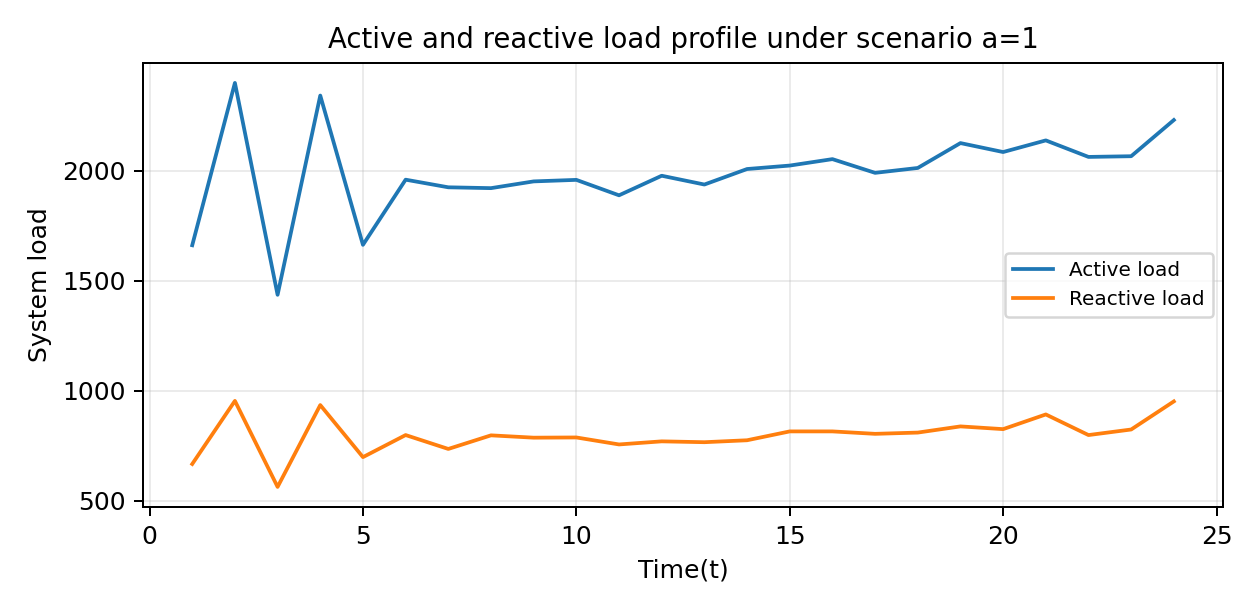
\includegraphics[width=0.48\textwidth]{docs/analysis_packs/assets/figures/scenario_profile_normal_load.png}
\caption{Active and reactive load profile under representative normal scenario
$a=1$.}
\label{fig:normal_load_profile}
\end{figure}

\begin{figure*}[t]
\centering
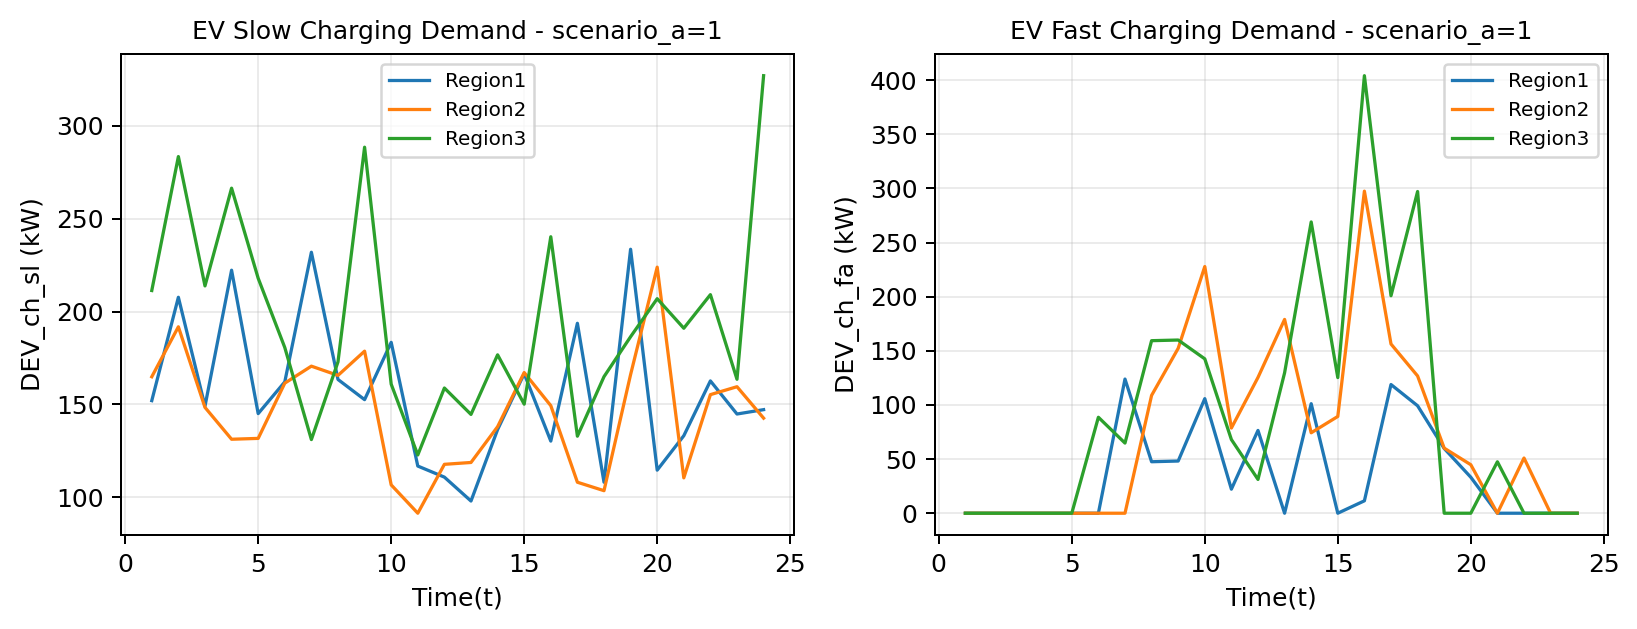
\includegraphics[width=0.78\textwidth,height=0.27\textheight,keepaspectratio]{docs/analysis_packs/assets/figures/scenario_profile_normal_ev_cropped.png}
\caption{Slow and fast EV charging demand profiles for each region under
representative normal scenario $a=1$.}
\label{fig:normal_ev_profile}
\end{figure*}

\begin{figure*}[t]
\centering
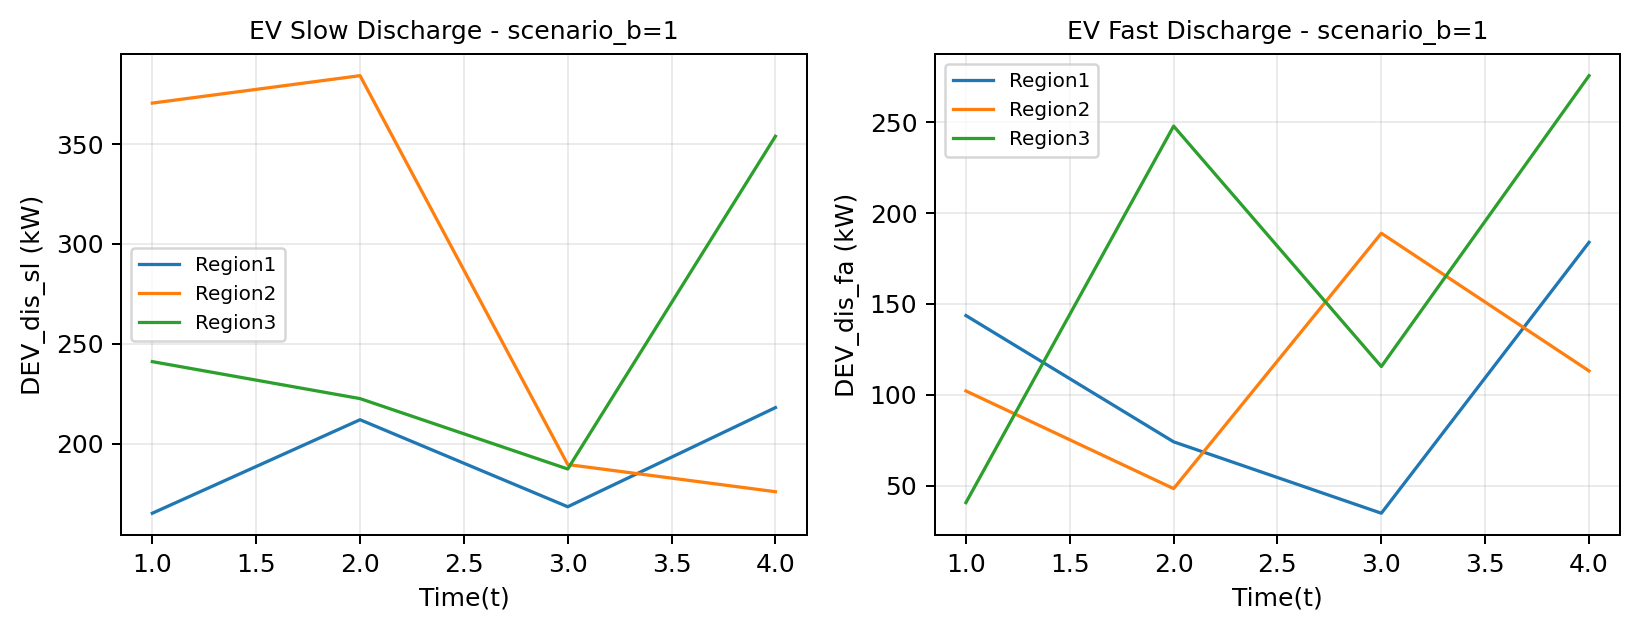
\includegraphics[width=0.78\textwidth,height=0.27\textheight,keepaspectratio]{docs/analysis_packs/assets/figures/scenario_profile_disaster_ev_cropped.png}
\caption{Slow and fast EV discharging availability profiles for each region
under representative disaster scenario $b=1$.}
\label{fig:disaster_ev_profile}
\end{figure*}

\subsection{Benchmark Definitions}
Four cases are designed to isolate the value of integrated stochastic
resilience planning. Case~1 is the proposed integrated DRO planner, which
jointly optimizes construction, normal-operation recourse, and disaster-stage
DRO recourse. Case~2 removes the disaster term and represents the
daily-service endpoint. Case~3 removes both the normal-stage EV service
objective and the normal-stage EV service constraints during training; it is a
resilience endpoint whose normal-service consequences are revealed only after
ex-post replay. Case~4 is a fair deterministic mean-value benchmark: it
replaces the multi-scenario normal and disaster profiles with their mean
profiles but keeps the same outage-budget semantics with $K_{\rm train}=2$.

The comparison is deliberately not based on the four training objectives.
After each case is solved, its first-stage siting and sizing decisions are
frozen and evaluated under the same $|A|=10$, $|B|=10$, $K_{\rm eval}=2$ MILP
worst-distribution evaluator. This common replay produces the component costs
reported below and is the basis for all cross-case claims.

\subsection{Default Component Comparison}
Fig.~\ref{fig:default_maps} shows the three endpoint planning maps used to
interpret the default comparison. Table~\ref{tab:default_components} reports
the objective decomposition:
$F^{\rm cons}$ is annualized construction cost, $F^{\rm trans}$ is EV user
transportation cost, $F^{\rm unmet}$ is unmet charging-demand penalty,
$F^{\rm sub}$ is substation purchase cost,
$\Psi^{\rm nor}=F^{\rm trans}+F^{\rm unmet}+F^{\rm sub}$ is the normal
component, and $\Phi^{\rm dis}$ is the worst-distribution disaster component.

\begin{figure*}[t]
\centering
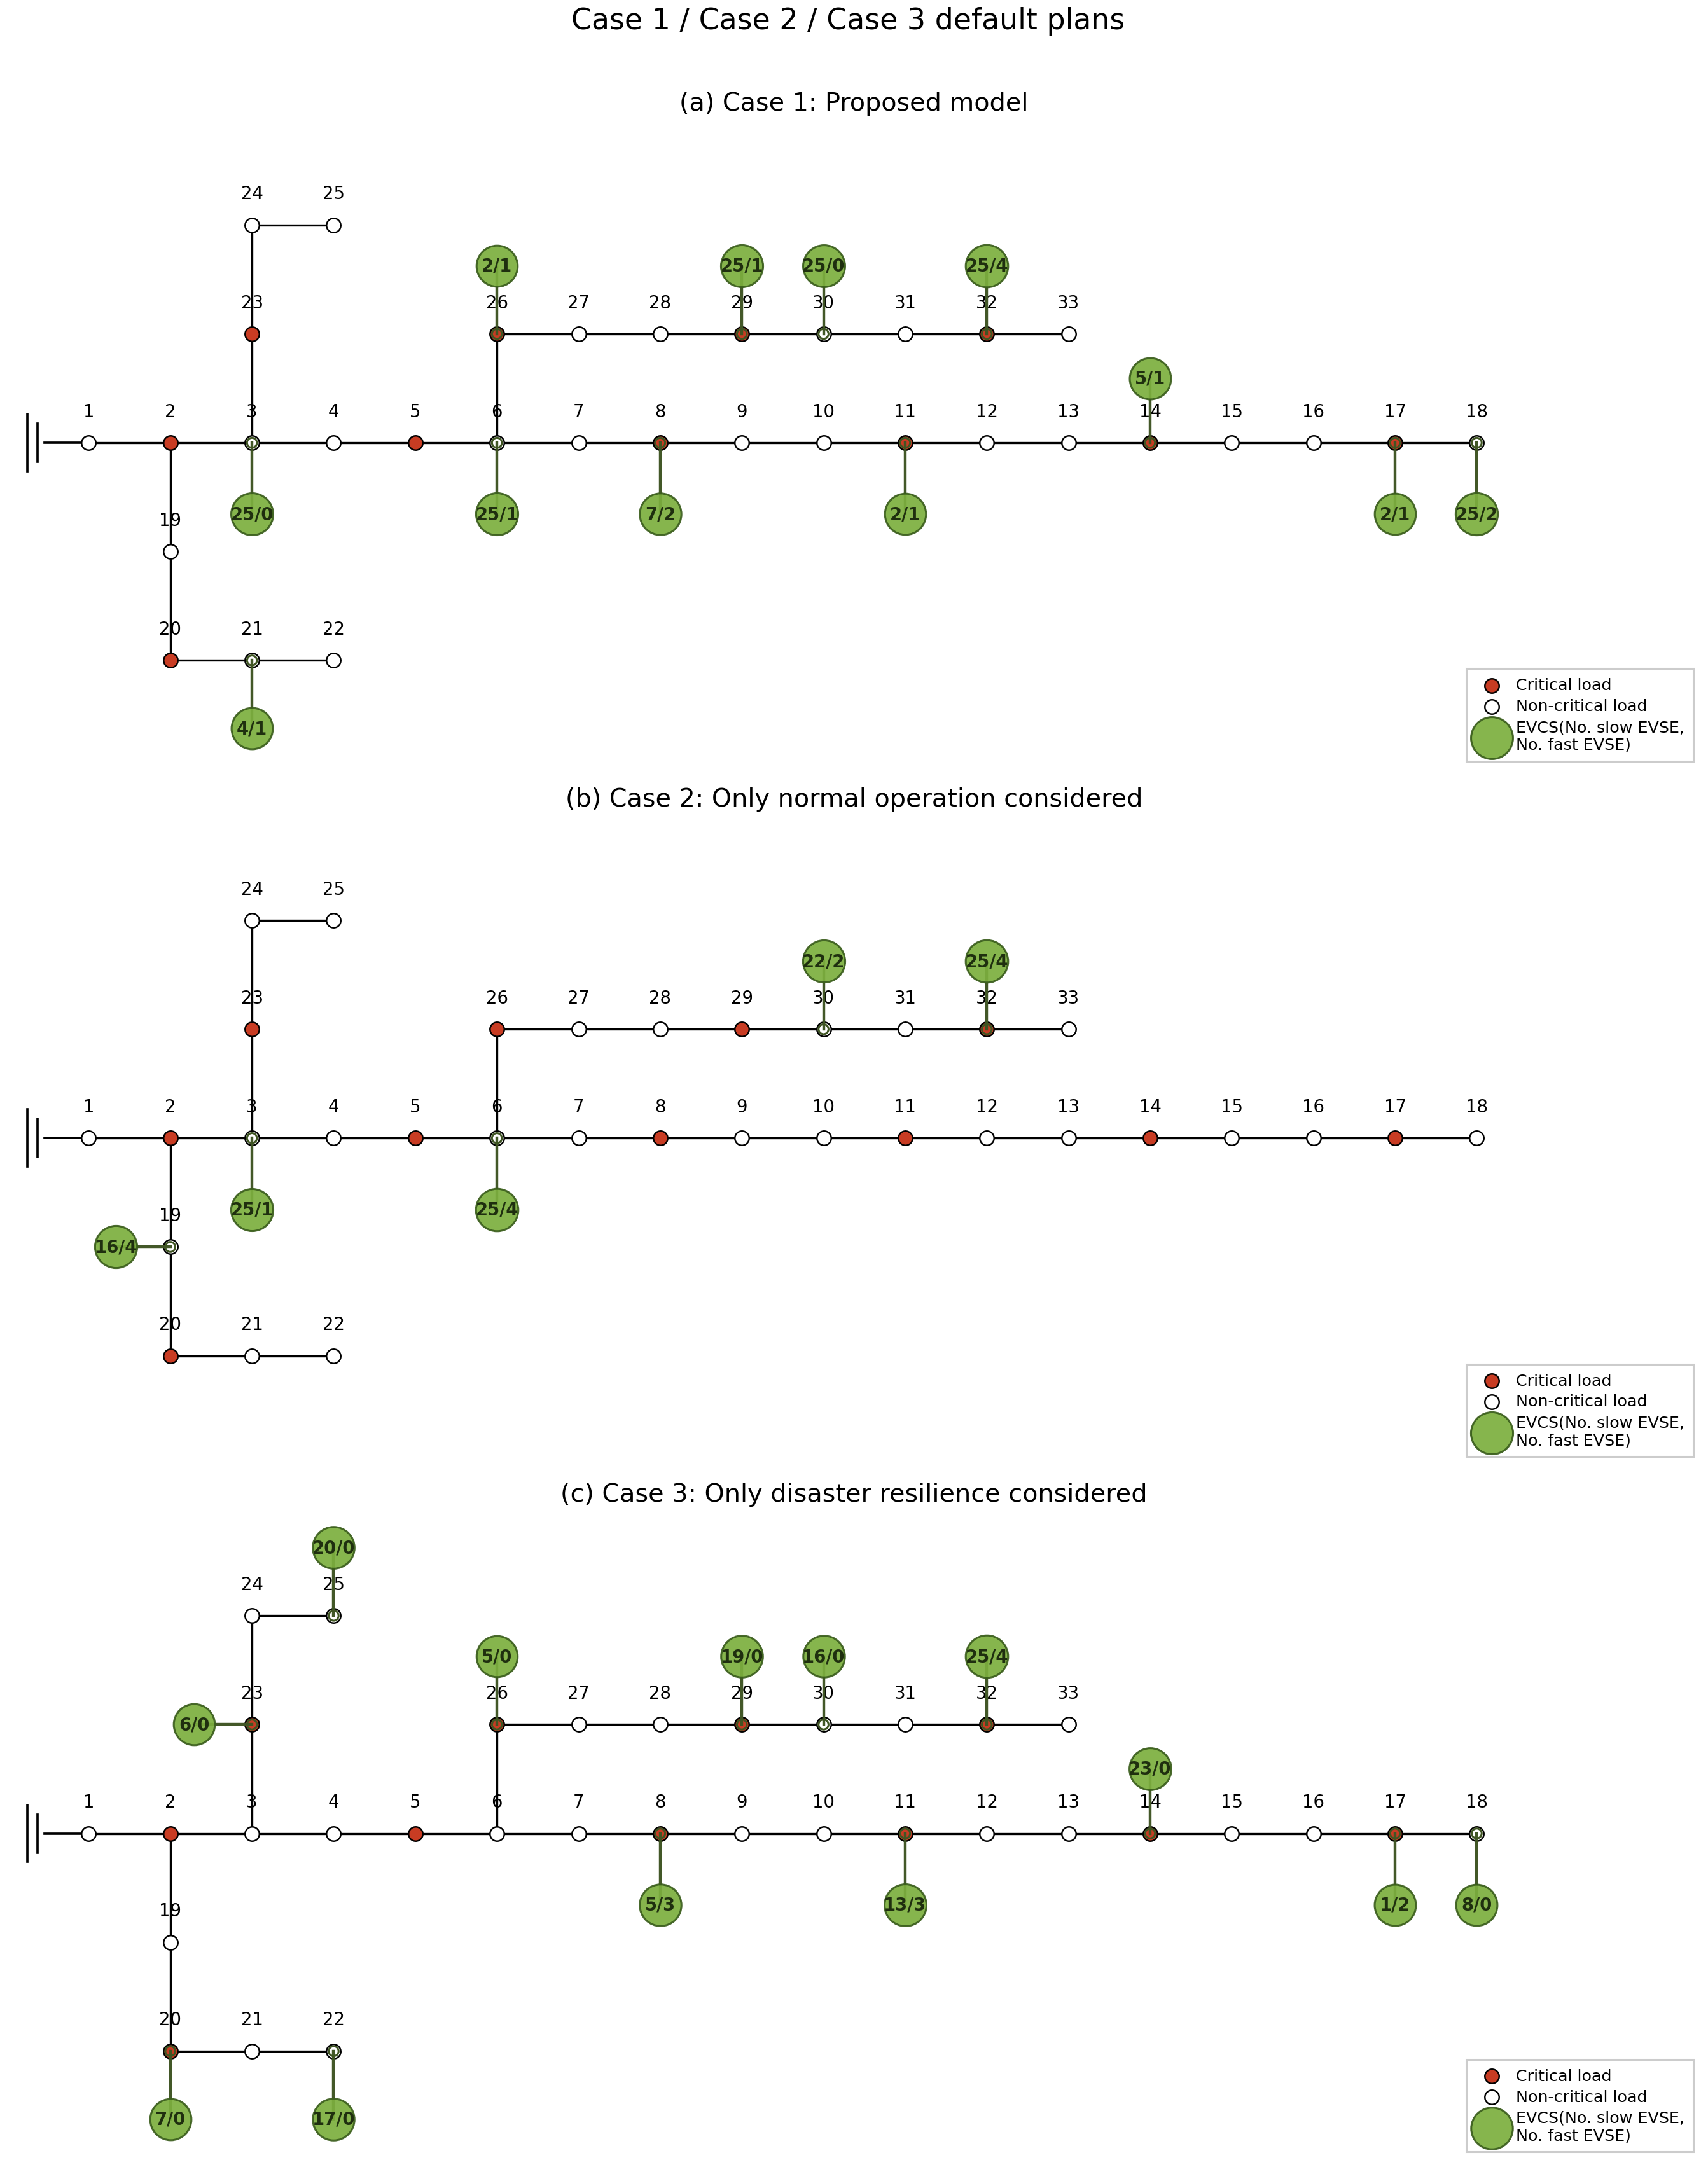
\includegraphics[width=0.86\textwidth,height=0.46\textheight,keepaspectratio]{docs/analysis_packs/assets/figures/fig6_like_plan_maps.png}
\caption{Planning maps for the proposed integrated, normal-only, and
disaster-only cases.}
\label{fig:default_maps}
\end{figure*}

\begin{table*}[t]
\centering
\caption{Objective components under the common $|A|=10$, $|B|=10$, $K=2$
MILP worst-distribution evaluator.}
\label{tab:default_components}
\begin{tabular}{lrrrr}
\toprule
Obj. (\$) & Case 1 & Case 2 & Case 3 & Case 4 \\
\midrule
$F^{\mathrm{cons}}$ & 128,069.89 & 66,721.59 & 132,216.04 & 104,765.26 \\
$F^{\mathrm{trans}}$ & 21,514.49 & 21,470.91 & 23,014.97 & 21,837.60 \\
$F^{\mathrm{unmet}}$ & 0.00 & 0.00 & 66,167.24 & 66,167.24 \\
$F^{\mathrm{sub}}$ & 40,809.78 & 40,809.78 & 40,769.87 & 40,769.87 \\
$\Psi^{\mathrm{nor}}$ & 62,324.28 & 62,280.70 & 129,952.07 & 128,774.70 \\
$\Phi^{\mathrm{dis}}$ & 5,223.70 & 16,774.96 & 4,358.42 & 6,545.72 \\
$J_{\mathrm{eval}}$ & 173,264.00 & 115,350.56 & 224,490.02 & 196,871.27 \\
Sites & 12 & 5 & 13 & 10 \\
Slow/Fast EVSE & 172/15 & 113/15 & 165/12 & 101/12 \\
Critical buses covered & 7/11 & 1/11 & 9/11 & 5/11 \\
\bottomrule
\end{tabular}
\end{table*}

Case~2 is the normal-service endpoint. It opens only five stations and keeps
zero unmet charging demand, so its normal component is almost identical to the
proposed plan: $\Psi^{\rm nor}$ is 62,280.70 in Case~2 and 62,324.28 in
Case~1. This small difference means that the integrated design does not buy
resilience by degrading daily EV service. The difference appears in the
disaster replay. Case~2 directly covers only 1/11 critical buses and has
$\Phi^{\rm dis}=16{,}774.96$, whereas Case~1 reduces the disaster component to
5,223.70. The integrated plan therefore lowers the normal-only disaster cost by
68.86\% while preserving zero unmet charging demand.

Case~3 is the disaster endpoint. It opens thirteen stations, directly covers
9/11 critical buses, and obtains the lowest disaster component,
$\Phi^{\rm dis}=4{,}358.42$. This confirms that the benchmark is genuinely
resilience-oriented. Its normal replay is poor: $F^{\rm unmet}=66{,}167.24$,
or 50.91\% of $\Psi^{\rm nor}$. The proposed plan lies between the two
endpoints. It keeps the normal-service quality of Case~2 and recovers most of
the resilience improvement of Case~3 without accepting the disaster-only
unmet-demand penalty.

The topology in Fig.~\ref{fig:default_maps} explains the mechanism. The
normal-only plan concentrates on daily-service anchors at buses 3, 6, 19, 30,
and 32. The integrated plan keeps daily anchors at buses 3, 6, 30, and 32, but
adds buses 8, 11, 14, 17, 18, 21, 26, and 29. These sites spread capacity
along the main feeder and the laterals, raising direct critical-bus coverage
from 1/11 to 7/11. The proposed design is therefore not just a larger version
of the normal-only plan; it shifts first-stage coverage toward critical-bus
neighborhoods while retaining low daily transportation and unmet-demand costs.

\subsection{Deterministic Mean-Value Comparison}
Case~4 isolates the value of multi-scenario DRO support from the value of the
outage budget itself. The deterministic benchmark is trained on mean normal and
mean disaster profiles, but it still uses $K_{\rm train}=2$; hence its
comparison with Case~1 is not a strawman without outage awareness.
Table~\ref{tab:det_worst} compares it with the proposed plan under the same
worst-distribution replay.

\begin{table*}[t]
\centering
\caption{Proposed and fair deterministic mean-value plans under the common
worst-distribution evaluator.}
\label{tab:det_worst}
\begin{tabular}{lrr}
\toprule
Metric & Proposed & Det. $K_{\rm train}=2$ \\
\midrule
$F^{\rm cons}$ & 128,069.89 & 104,765.26 \\
$\Psi^{\rm nor}$ & 62,324.28 & 128,774.70 \\
$\Phi^{\rm dis}$ & 5,223.70 & 6,545.72 \\
$\pi_f\Phi^{\rm dis}$ & 1,567.11 & 1,963.72 \\
$J_{\rm eval}$ & 173,264.00 & 196,871.27 \\
Sites & 12 & 10 \\
Slow/Fast EVSE & 172/15 & 101/12 \\
Critical buses covered & 7/11 & 5/11 \\
Reduction in $\Phi^{\rm dis}$ & -- & 20.20\% \\
\bottomrule
\end{tabular}
\end{table*}

The deterministic plan is a fair comparator because it has the same
outage-budget semantics as the proposed model. Its weakness is that the mean
profiles do not represent the multi-scenario tails used in the common replay.
It opens ten stations and installs 101 slow and 12 fast EVSEs, whereas the
proposed DRO plan opens twelve stations and installs 172 slow and 15 fast
EVSEs. The additional capacity is spatially meaningful: Case~1 expands
coverage around buses 17, 21, and 26 and strengthens the upper lateral through
buses 29, 30, and 32. Under the common worst-distribution replay, this broader
topology reduces $\Phi^{\rm dis}$ from 6,545.72 to 5,223.70, a 20.20\%
reduction. The evaluated total cost also falls from 196,871.27 to 173,264.00,
because the deterministic first-stage saving is outweighed by poorer common
replay performance.

\subsection{EV Penetration Sensitivity}
The EV penetration study scales both normal charging demand and disaster V2G
availability by 2.0 and 3.0 while keeping the economic parameters, objective
multipliers, $|A|=10$, $|B|=10$, and $K=2$ fixed. Fig.~\ref{fig:ev_sensitivity_maps}
shows the resulting plans, and Table~\ref{tab:ev_sensitivity} reports the same
component taxonomy used in the default comparison.

\begin{figure*}[t]
\centering
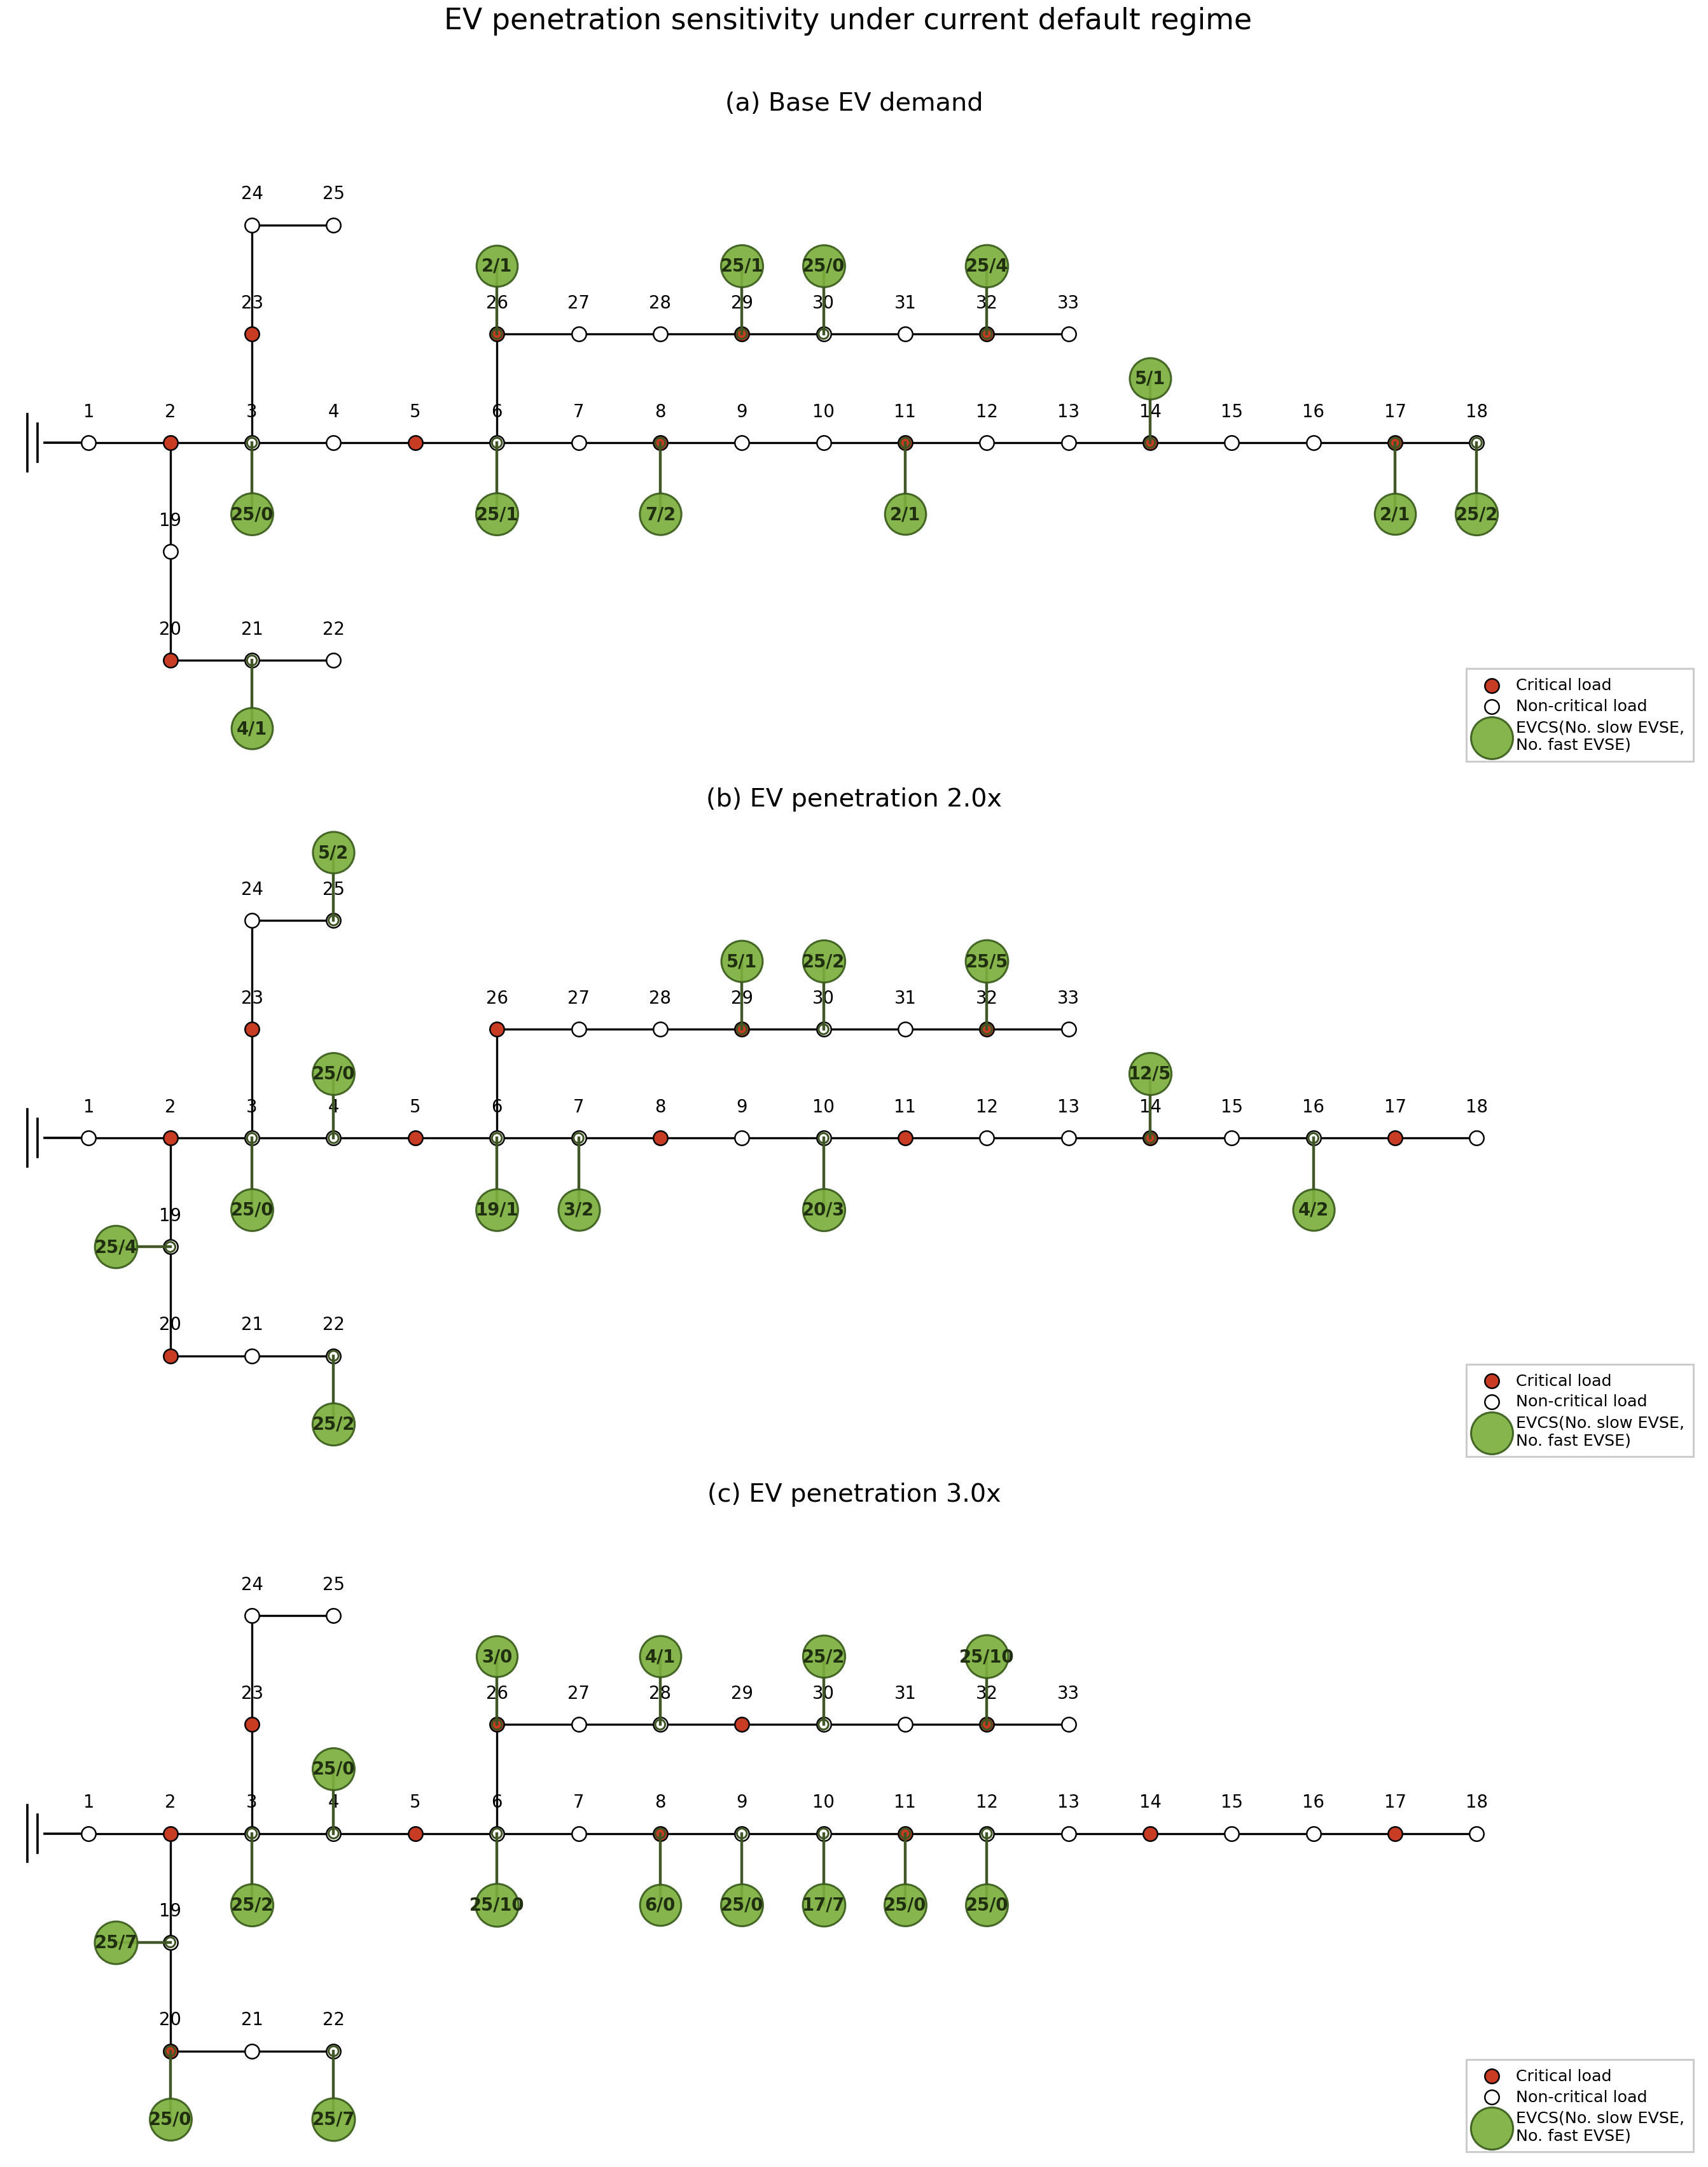
\includegraphics[width=0.78\textwidth,height=0.50\textheight,keepaspectratio]{docs/analysis_packs/assets/figures/fig8_like_sensitivity_maps.png}
\caption{Planning maps for the base, 2.0x EV, and 3.0x EV penetration cases.}
\label{fig:ev_sensitivity_maps}
\end{figure*}

\begin{table*}[t]
\centering
\caption{EV penetration sensitivity under the default setting.}
\label{tab:ev_sensitivity}
\begin{tabular}{lrrr}
\toprule
Metric & Base & EV 2.0x & EV 3.0x \\
\midrule
$F^{\mathrm{cons}}$ & 128,069.89 & 157,353.74 & 200,532.58 \\
$F^{\mathrm{trans}}$ & 21,514.49 & 43,389.32 & 65,361.34 \\
$F^{\mathrm{unmet}}$ & 0.00 & 0.00 & 0.00 \\
$F^{\mathrm{sub}}$ & 40,809.78 & 51,193.18 & 61,576.58 \\
$\Psi^{\mathrm{nor}}$ & 62,324.28 & 94,582.51 & 126,937.92 \\
$\Phi^{\mathrm{dis}}$ & 5,223.70 & 3,299.38 & 4,811.99 \\
$J_{\mathrm{eval}}$ & 173,264.00 & 224,551.31 & 290,832.72 \\
Sites & 12 & 13 & 15 \\
Slow/Fast EVSE & 172/15 & 218/29 & 305/46 \\
Rated EVSE capacity (kW) & 1,954 & 2,976 & 4,435 \\
Critical buses covered & 7/11 & 3/11 & 5/11 \\
\bottomrule
\end{tabular}
\end{table*}

The model absorbs the larger EV population without unmet charging demand in
all three cases. The normal components increase for physical reasons:
$F^{\rm trans}$ rises with the larger charging population, and
$F^{\rm sub}$ rises from 40,809.78 to 61,576.58 as served energy increases.
The first-stage capacity response is monotone. Open sites increase from 12 to
13 and 15, the slow/fast EVSE mix expands from 172/15 to 218/29 and 305/46,
and rated EVSE capacity rises from 1,954~kW to 2,976~kW and 4,435~kW. The
3.0x case is therefore not solved by suppressing charging demand; it is solved
by expanding both spatial coverage and charger capacity.

The disaster component remains controlled under the same common replay. It
decreases to 3,299.38 in the 2.0x case because the larger EV fleet also
provides additional V2G availability. At 3.0x, $\Phi^{\rm dis}$ rises to
4,811.99 relative to the 2.0x row, but it remains below the base value while
the system serves a much larger charging population with zero unmet demand.
This pattern is consistent with a capacity-expansion interpretation: additional
infrastructure and V2G support offset much of the increased operating burden.

\subsection{Computational Scalability and Convergence}
The computation study separates two uncertainty dimensions. The disaster
support size $|B|$ increases the number of operating-condition profiles that
must be priced in the separation problem. The outage budget $K$ increases the
combinatorial ambiguity set over line outages and therefore changes the
closure difficulty of the Benders loop. All results in this subsection use the
same default economic setting and MILP separation.

\begin{center}
\refstepcounter{figure}\label{fig:k_convergence_runtime}
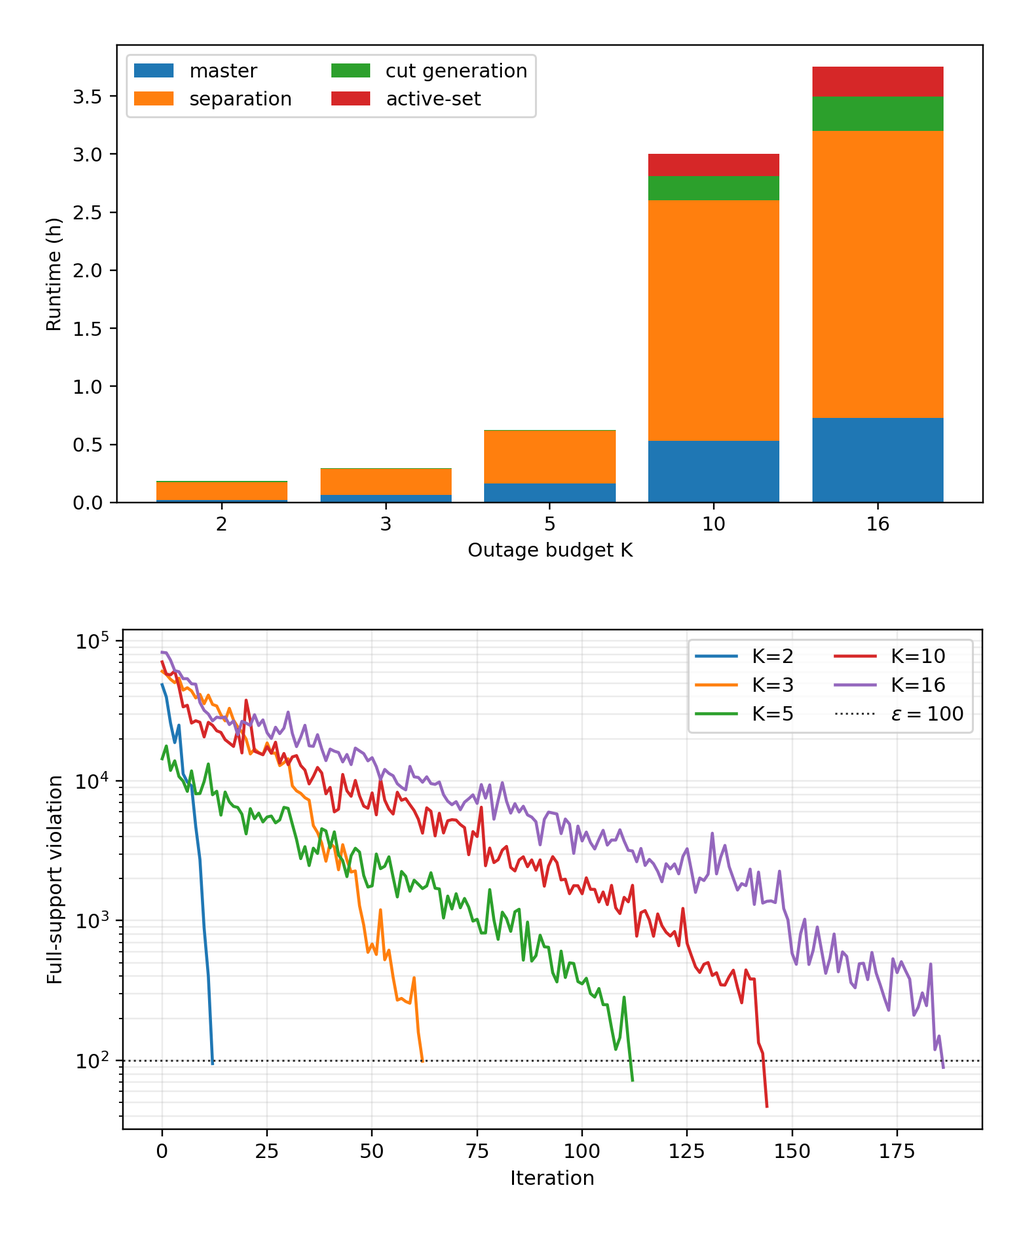
\includegraphics[width=\columnwidth,height=0.35\textheight,keepaspectratio]{docs/analysis_packs/assets/figures/current_default_k_convergence_runtime_column.png}
\parbox{0.96\columnwidth}{\footnotesize
Fig.~\thefigure. Runtime decomposition and full-support violation traces for
outage-budget scaling. The stacked bars show that separation dominates the
large-$K$ runtime, while the violation traces show the Benders closure toward
the common $\epsilon=100$ certificate threshold.}
\end{center}

\begin{table}[!t]
\centering
\caption{Disaster-support scalability with $|A|=10$ and $K=2$.}
\label{tab:b_scaling}
\scriptsize
\begin{tabular}{rrrrrrl}
\toprule
$|B|$ & $t$ (h) & Sep. & It. & Cuts & Viol. & Cert. \\
\midrule
5 & 0.11 & 33.3\% & 43 & 126 & 31.43 & $\epsilon$ \\
10 & 0.11 & 62.0\% & 37 & 107 & 91.67 & $\epsilon$ \\
20 & 0.35 & 79.1\% & 41 & 120 & 83.90 & $\epsilon$ \\
50 & 1.33 & 94.9\% & 38 & 110 & 23.59 & $\epsilon$ \\
\bottomrule
\end{tabular}
\end{table}

Table~\ref{tab:b_scaling} shows that full planning is certified through
$|B|=50$ under the current default regime. The iteration counts stay between
37 and 43 for the certified rows, while the runtime increases from 0.11~h at
$|B|=5$ to 1.33~h at $|B|=50$. The reason is visible in the decomposition:
the separation share grows from 33.3\% to 94.9\%. Thus, increasing $|B|$ does
not mainly increase the number of Benders iterations; it makes each
full-support separation call more expensive. The one-shot separation results
show the same trend and confirm that the separation oracle remains optimal
over the certified support range.

\begin{table}[!t]
\centering
\caption{Certified outage-budget record with $|A|=10$ and $|B|=10$.}
\label{tab:k_scaling}
\scriptsize
\begin{tabular}{llrrrr}
\toprule
$K$ & Algorithm path & Cert. & It. & Viol. & $t$ (h) \\
\midrule
2 & mainline & $\epsilon$ & 13 & 94.96 & 0.18 \\
3 & mainline & $\epsilon$ & 63 & 98.76 & 0.30 \\
5 & continuation & $\epsilon$ & 113 & 72.27 & 0.62 \\
10 & accelerated & $\epsilon$ & 146 & 47.00 & 3.00 \\
16 & accelerated & UB gap & 187 & 89.31 & 3.75 \\
\bottomrule
\end{tabular}
\end{table}

Table~\ref{tab:k_scaling} and Fig.~\ref{fig:k_convergence_runtime} give the
certified outage-budget record and convergence behavior. The $K=2$, 3, and 5
rows are small- and medium-budget baselines. The direct apple-to-apple
comparison is between $K=10$ and $K=16$, which both use the same active-set
and target-face cut-generation configuration. Increasing $K$ from 10 to 16
raises certified runtime from 3.00~h to 3.75~h and cuts from 1,016 to 1,307.
The $K=10$ row closes by an ordinary full-support $\epsilon$ certificate,
whereas $K=16$ closes with a pricing-derived upper bound and canonical lower
bound; the gap is 37.51, below the same $\epsilon=100$ threshold. The
violation traces show the same certificate closure pattern.
